\documentclass{article}
\usepackage[utf8]{inputenc}
\usepackage{amsmath, amssymb}
\usepackage{mathtools}
\usepackage{graphicx}
\usepackage[textwidth=18cm, textheight=26cm]{geometry}
\usepackage{gensymb}
\usepackage{enumitem}

%\documentclass[12pt]{report}

\title{ME 270 Final Presentation \\The Able Table}
\author{Vedant Puri, Team ABD I}
\date{April 28, 2017}

\begin{document}
\maketitle

\textbf{The ``Cam'' Mechanism}\\ We are using a variable radium pulley, or a ``cam,'' that is maintained in equilibrium, so as to have it rotate freely. The cam would eat or release slack in the cable wrapped on it. Changing the length of slack would then change the height of the table.
Conversely, applying a force to, say, lift the table would reduce the tension in the cables. The cams would rotate to maintain equilibrium and eat slack in the cable to reduce the space between the legs, which would lift the table surface up.

\bigskip

\\\textbf{The Mathematics} \\ The objective is to maintain the cam in equilibrium at all angles, so it would be able to rotate freely. This is done by varying the radius, and hence varying the moment caused by cable tension. Using a spring to counter the torque caused by cable tension, we seek an equation relating the radius of the cam to the angle of rotation, $\alpha$.

\begin{center}\bigskip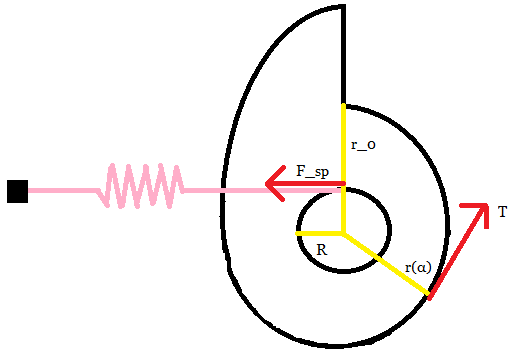
\includegraphics[scale=0.5]{cam.png}\\\textbf{Figure 1: Schematic of variable radius pulley.} \end{center}

$$M_{\text{spring}}=M_{\text{Tension}}$$
At angle $\alpha=0$, the radius of the pulley is $r_0$. For arbitrary angle $\alpha\in[0,2\pi]$,
\begin{equation}
Tr(\alpha)=Rkx(\alpha)
\end{equation}
Moving forward by an angle $\text{d}\alpha$,
\begin{equation}
    Tr(\alpha+\text{d}\alpha)=Rkx(\alpha+\text{d}\alpha) 
\end{equation}

\begin{center}\bigskip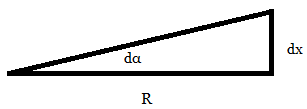
\includegraphics[scale=0.5]{angle.png}\\\textbf{Figure 2: Relation between d$\alpha$ and dx.} \end{center}

From Figure $2$,
\begin{equation}
    \text{d}x=x(\alpha+\text{d}\alphaa)-x(\alpha)=R\tan{\text{d}\alpha}
\end{equation}

\newpage

For small $x$, $\tan{x}\approx x$. Combining equations (1), (2) and (3),
\begin{equation}
    r(\alpha+\text{d}\alpha)-r(\alpha)=\frac{Rk}{T}R\text{d}\alpha
\end{equation}
Taking the limit $\text{d}\alpha \to 0$,
\begin{equation}
    \lim_{\text{d}\alpha \to 0}\frac{r(\alpha+\text{d}\alpha)-r(\alpha)}{\text{d}\alpha}=\frac{R^2k}{T}=\frac{\text{d}r}{\text{d}\alpha}
\end{equation}
Solving the differential equation (5) with initial condition stated above,
\begin{equation}
    r(\alpha)=r_0+\frac{R^2k}{T}\alpha
\end{equation}

\textbf{Result}\\The cam radius, therefore, linearly increases as angle increases from zero to $2\pi$. From our table design, however tension (T) turns out to be highly non-linear, and could not be easily measured. We performed multiple Design of Experiment (DOE) trials, by varying R and spring constant k to find the arrangement that maximizes range. For the final cam, we chose the initial radius to be $r_0=1$ in, the final radius to be $4$ in and $R$ to be $1.5$ in. To go with that, we chose a spring of constant $4.8$ lb$/$in. For these values of $k$ and $R$, we are expecting a tension $T$ value of approximately (using equation ($6$) $22.6$ lb.
\end{document}